% !TEX root = Thesis.tex

\chapter{Layout Extraction and Preservation}\label{chap:LayoutExtPre}

  In this chapter, we emphasis on how to decompose the analog layout in placement and routing. We first divide the layout with blocks and wire segments, and later extract them respectively. The overall extraction flow is illustrated as Fig.~\ref{fig:ExtractFlow}. 

  \begin{figure}[t]
    \centering
    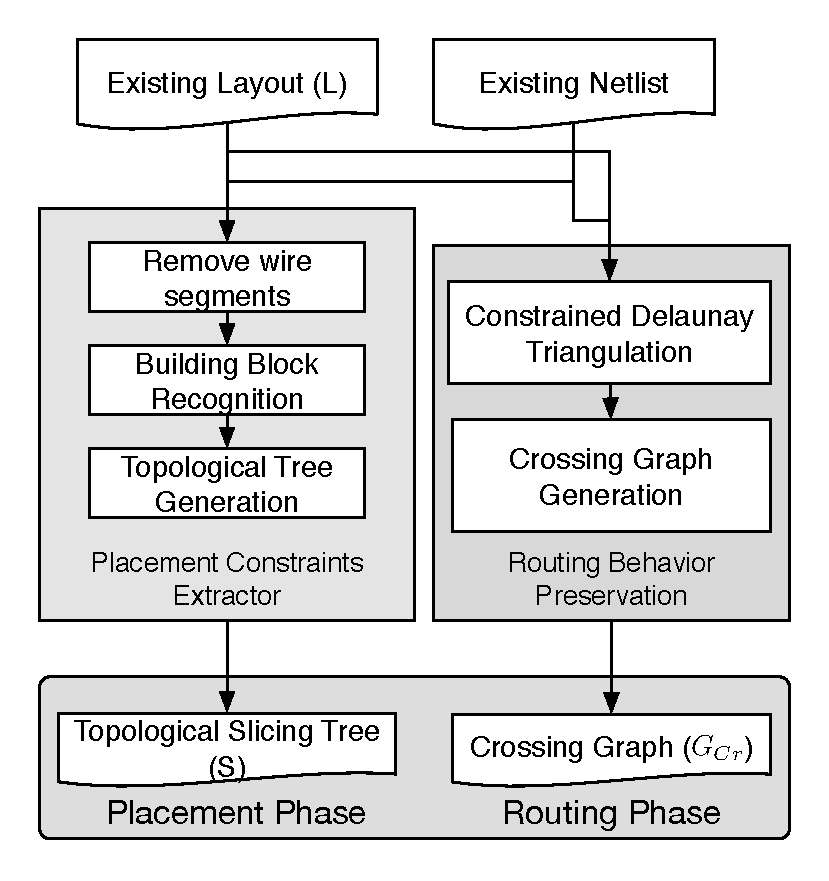
\includegraphics[height=7cm]{Fig/ExtractFlow.eps}
    \caption{The extraction separates layout into placement phase as topological slicing tree and as routing phase crossing graph.}
    \label{fig:ExtractFlow}
  \end{figure}


  \section{Placement Constraints Extraction}\label{sec:PlExtract}

    \begin{figure}[t]
      \begin{center}
      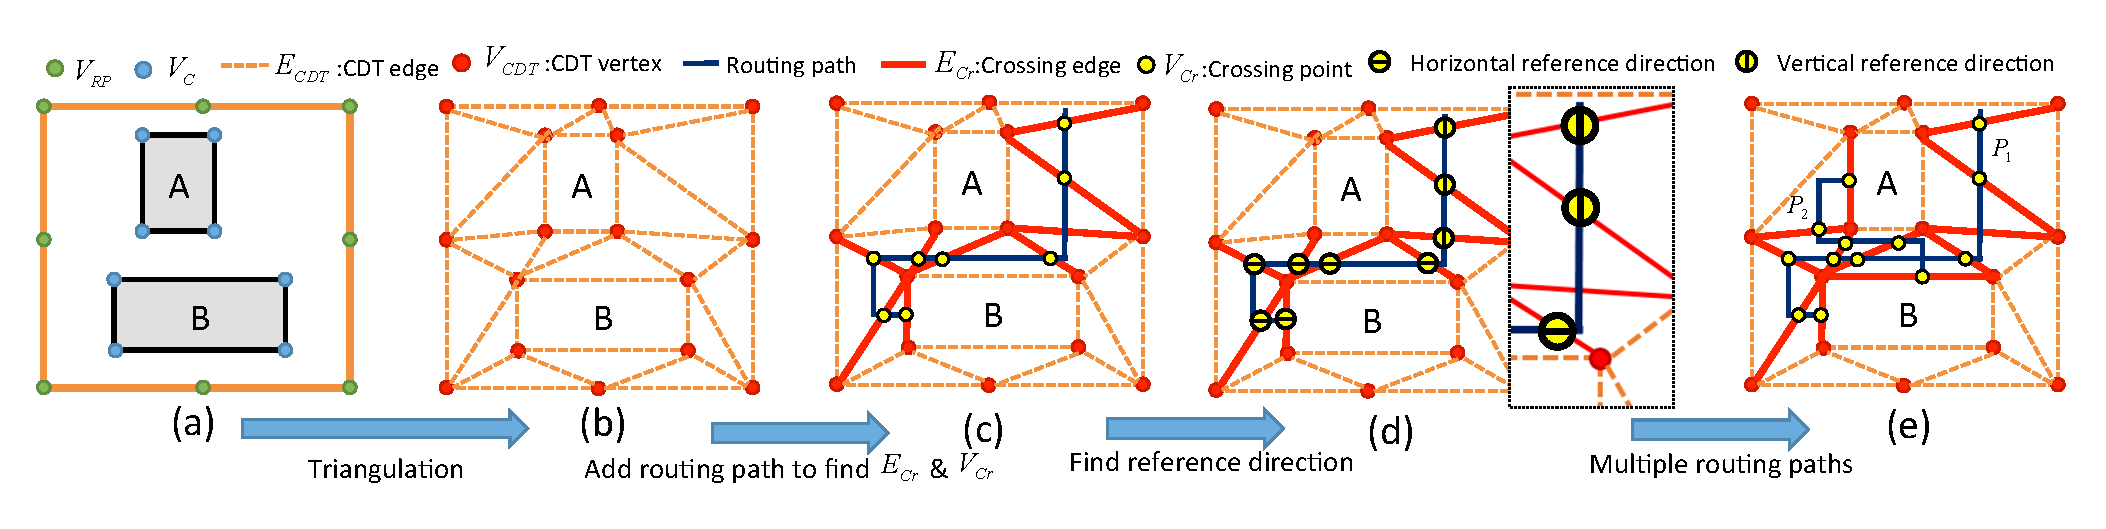
\includegraphics[width=\textwidth]{Fig/CGC.eps}
      \caption{Illustration of routing preservation by CDT. 
        (a) The given design.
        (b) Resultant CDT graph $G_{CDT}$.
        (c) CDT edges crossing with routing path are colored by red.
        (d) Crossing points of the two paths in routing plane.
        (e) Routing behavior is stored by CDT graph and the crossing points.}
      \label{fig:CGC}
      \end{center}
    \end{figure}

    %In the beginning of placement constraints extraction, we first remove the wire segments from the existing layout then implement extraction. 
    The major flow of placement constraints extraction \cite{ALP_YPWeng_iccad2011} is reviewed as follows:
    \subsection{Building Block Recognition}
      In order to reduce mismatch while generating layout, the principles of symmetrical and matching constraints should be considered as building blocks. 
      Besides, Building blocks under the same matching constraints are identified by the existing netlist. Via pattern matching technique \cite{Massier_TCAD08} the preferable matching building blocks are generated.

    \subsection{Topological Slicing Tree Generation}
      Later, these fundamental build blocks construct the topological slicing tree. In general, the placement can be decomposed by horizontal and vertical cuts. However, since some of the devices are recognized as build blocks, the traditional slicing tree tends to occur mismatches. Instead, cells under the same building block are placed together as a super-module in representation. After vertical and horizontal  partitioning, a topological slicing tree (S) with n symmetry groups, m matching groups which outside any symmetry group, and l non-symmetry cells in layout are generated at the same hierarchy. Other than \cite{ALP_YPWeng_iccad2011} which flattens the layout into the unit hierarchy for slicing tree generation, we preserved the hierarchy of the layout with respect to the hierarchical structure from the existing netlist. Such hierarchy is essential for multi-level layout reconstruction. 




  \section{Routing Preservation via Crossing Graph Construction}\label{sec:CGC}


    \newcommand{\CCG}{\ensuremath{\mbox{\sc ConstCrossGraph}}}
    \begin{algorithm}[hbt]  
      \caption{$\CCG(P,B,V_{RP})$}\label{alg:CCG}                       
      \begin{scriptsize}
        \begin{algorithmic}[1]
          \REQUIRE 
            \begin{tabular}{l}
              $P$: The routing paths of layout\\
              $B$: The placement blocks \\
              $V_{RP}$: Corners of layout and the middle-points of each plane boundary\\ 
            \end{tabular}
          \ENSURE 
            \begin{tabular}{l}
              $T$: The triangles after CDT\\
              $E_{CDT}$: The edges set of $G_{CDT}$\\
              $V_{Cr}$: The set of crossing points between routing paths and $E_{CDT}$\\
              $E_{Cr}$: The set of crossing edge\\
              $G_{Cr}$: The crossing graph
            \end{tabular}
          \FOR {$i = 1 \to |B|$}
            \STATE $V_C \gets v^{TR},v^{TL},v^{BR},v^{BL} $ \COMMENT{collect four corners into $V_C$}
          \ENDFOR
          \STATE $V_{CDT}\gets V_C, V_{RP}$  \label{line:VCDT}
          \STATE $G_{CDT}(V_{CDT},E_{CDT},B,T) \gets CDT(V_{CDT},B)$  \COMMENT{constrained Delaunay triangulation} \label{line:GCDT}
          \FOR {$i = 1 \to |P|$} \label{line:StartCross}
            \STATE $E_{Cr}(p_i) \gets CheckCrossEdge(p_i,E_{CDT})$
            \FOR {$j = 1 \to |E_{Cr}(p_i)|$}
              \STATE $v(x,y) \gets FindCross({E_{Cr}(p_i)}_j)$
              \STATE $q_1,q_2 \gets FindAdjacent({E_{Cr}(p_i)}_j,V_{CDT})$
              \STATE $V_{Cr}(p_i) \gets v,q_1,q_2$
            \ENDFOR
            \STATE $E_{Cr} \gets E_{Cr}(p_i)$
            \STATE $V_{Cr} \gets V_{Cr}(p_i)$
          \ENDFOR \label{line:EndCross}
          \RETURN $G_{Cr}(V_{CDT}\cup V_{Cr}, E_{CDT} \cup E_{Cr},B,T)$  
        \end{algorithmic}
      \end{scriptsize} 
    \end{algorithm}

    This Section introduces a new representation to preserve the routing correlation with placement. As Fig.~\ref{fig:WhyCDT}.(a) illustrated, the routing channel can be decomposed into multiple triangles via CDT. Thus, the wire goes across one or more triangles on their edges. The representation which aims to record the "crossing" behavior among wires and triangular edges is denoted by a crossing graph. The crossing graph construction is demonstrated in the following paragraph. 


    Fig.~\ref{fig:CGC} illustrates a routing preservation procedure and Algorithm~\ref{alg:CCG} {\it ConstCrossingGraph} represents it as a pseudocode. Given a layout plane $L$ with a set of placement blocks $B \in L$, where $B = \{b_i|1 \leq i \leq |B|\}$. As the layout without routing path shown in Fig.~\ref{fig:CGC}.(a), the set of corner points of blocks in $B$ are denoted by $V_C$ where $V_C = \{(x_i,y_i)|1 \leq i \leq 4|B|\}$, and the points on the periphery of routing plane (i.e. corners of the routing plane and the middle-points of each routing plane boundary) are denoted by $V_{PR}$. We define the vertex set of the layout extraction CDT to be $V_{CDT} = V_C \cup V_{RP}$ in line~\ref{line:VCDT}. Regions that forbid CDT edge are called {\it blocks} in CDT formulations. In our case, they are the areas inside blocks.


    As shown in line~\ref{line:GCDT}, the CDT graph $G_{CDT}$ generated from vertex set $V_{CDT}$ and block set $B$ can be represented as $G_{CDT} = \{V_{CDT},E_{CDT},B,T\}$, where the edge set $E_{CDT} = \{(v_i,v_j)|v_i,v_j\in V_{CDT}\}$ splits the plane into a set of non-overlapping triangles $T$ and the rectangular blocks $B$. According to Fig.~\ref{fig:CGC}.(b), the layout with 2 blocks are transferred into a $G_{CDT}$ after triangulation, where $|B|$=2 (block A and B), $|V_{CDT}|=16$, $|E_{CDT}|=34$ and $|T|=18$.


    After $G_{CDT}$ is established, one routing path is recovered back to demonstrate the routing preservation. As displayed in Fig.~\ref{fig:CGC}.(c), one $e_{CDT}$ intersects with the routing path is denoted by a crossing edge $e_{Cr}$ and the intersected point is denoted by a crossing point $v_{Cr}$. The detailed definition is as follows:

     
    \begin{defi}\label{defi:CrossingPoint}
      Given a routing path $p$, and CDT edge set $E_{CDT}= \{e_{CDTi}| 1 \leq i\leq|E_{CDT}|\}$, if there exists a point $v(x,y)$ which is both on $p$ and $e_{CDTi}$, $e_{CDTi}$ is a crossing edge $e_{Cr}$ and $v(x,y)$ is a crossing point $v_{Cr}$.
    \end{defi}

    From line~\ref{line:StartCross} to line~\ref{line:EndCross} in Algorithm~\ref{alg:CCG}, the procedure traverses the set crossing edges $E_{Cr}$ and crossing points $V_{Cr}$ is delivered. As Fig.~\ref{fig:CGC} displayed, an orange dotted line which originally denotes $e_{CDT}$ changes into solid red line as a crossing edge $e_{Cr}$, and the yellow point represents the intersection between the routing path, and such intersected point denotes a crossing point $v_{Cr}$. In addition, each $v \in V_{Cr}$ belongs to a routing path along with a crossing direction (horizontal/vertical, H/V), as illustrated in Fig.~\ref{fig:CGC}.(d). The directions are treated as {\it reference directions} which will be used later in the routing reconstruction stage, described in Section~\ref{chap:prototyping}. 



    For multiple nets design, a single edge might be crossed with two or more routing paths. As illustrated in Fig.~\ref{fig:CGC}(e), the two routing paths, $p_1$ and $p_2$, both pass through space between block A and B with $p_2$ closer to block A. In order to preserve the behavior of multiple nets routing, we define the {\it crossing graph} $G_{Cr}$ of layout $L$ as follows:
    \vspace{0.2cm}
    \begin{defi}\label{defi:CrossGraph}
      Let $G_{CDT}(V_{CDT},E_{CDT},B,T)$ denotes the CDT graph of $L$. $V_{Cr}$ denotes the set of crossing point and $E_{Cr}$ denotes the set of crossing edges. Then graph $G_{Cr} = \{V_{CDT} \cup V_{Cr},E_{CDT} \cup E_{Cr},B,T\}$ is a crossing graph of layout $L$. 
    \end{defi}
    \vspace{0.2cm}
    In the end, the crossing graph stores not only the individual routing topology, but also the relative order of paths within each routing channel.


  \section{Hierarchical Layout Extraction and Preservation}\label{sec:HLE}

    \begin{figure}[t]
      \begin{center}
      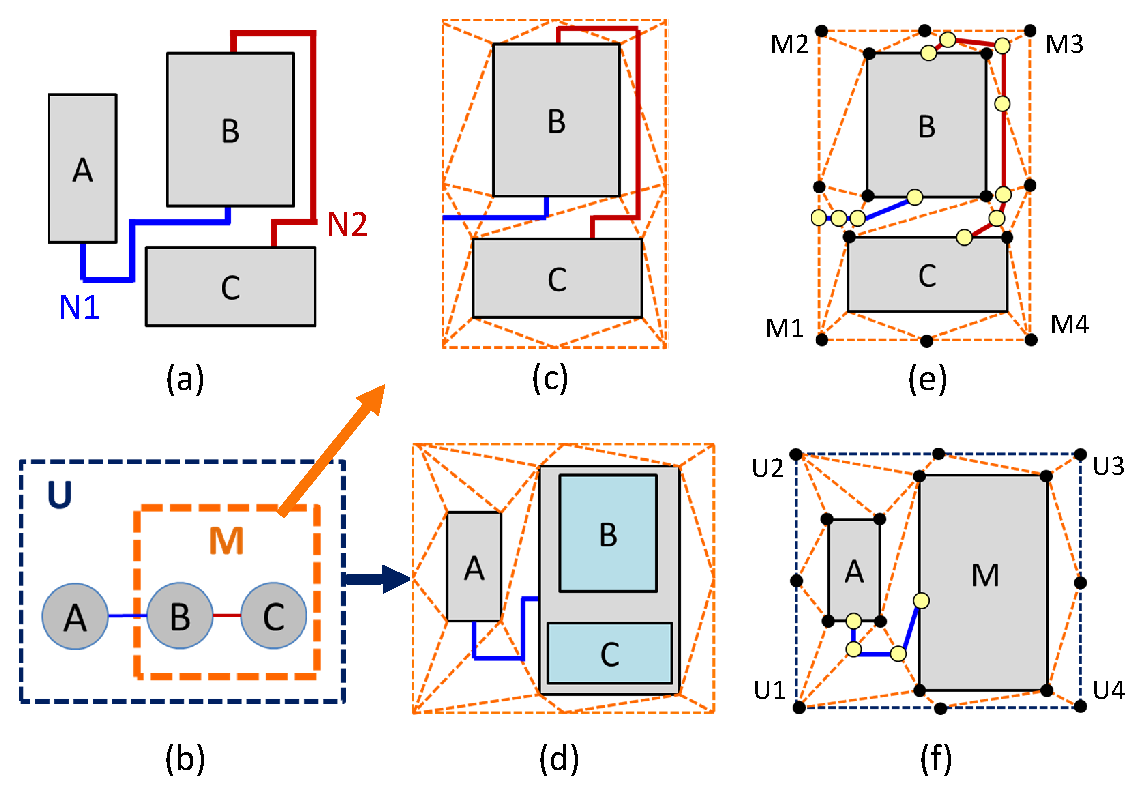
\includegraphics[width=8.5cm]{Fig/HIER.eps}
      \caption{
         (a) A layout with 3 placement blocks and two routing paths. 
         (b) Hierarchical Structure of (a).
         (c) CDT graph of cluster M (bottom level cluster).
         (d) CDT graph of cluster U (upper level cluster).
         (e) Corresponding crossing graph of (c).
         (f) Corresponding crossing graph of (d), cluster M is regarded as a placement block here.
        }
      \label{fig:HIER}
      \end{center}
    \end{figure}

    In order to reduce mismatches, the symmetry and proximity constraints need to be considered for both placement and routing. 
    For the given source layout, modules/devices are grouped as clusters according to the symmetry and proximity constraints, 
    where the constraints can be either given by designers or extracted from the source layout as in Section~\ref{sec:PlExtract}.

    For each cluster, the routing behavior and correlation with placement blocks are analyzed based on the CDT of that cluster to build a corresponding crossing graph. 
    Crossing graphs of clusters are constructed bottom-up along the hierarchical structure. 
    Bottom-level clusters are regarded as placement blocks in upper-level clusters. 
    Consequently, a series of crossing graphs is generated which contain the routing behavior hierarchically.

    Fig.~\ref{fig:HIER} illustrates this multilevel crossing graph generation.
    Fig.~\ref{fig:HIER}(a) shows a simple layout with three blocks and two nets.
    Assume block B and C are grouped into cluster M, and M and A are grouped into U as shown in Fig.~\ref{fig:HIER}(b).
    According to the hierarchy, two crossing graphs are constructed with respect to cluster M and U, and
    each routing path is divided into 1) intra-cluster connections and 2) inter-cluster connections. 
    As illustrated in Fig.~\ref{fig:HIER}(c)(d), path N1 is segmented into inside parts and outside parts of M. 
    Therefore, the crossing points of N1 appear in both two crossing graphs. 
    On the other hand, since N2 contains only intra cluster connection in M, the corresponding crossing points are all inside a single graph. 

    

